\documentclass[11pt]{article}
\usepackage{graphicx}
\usepackage[legalpaper,landscape, margin=0.4in]{geometry}
\usepackage{multicol}
\usepackage{titlesec}

\titlespacing*{\subsection}
{0pt}{1ex plus 1ex minus .3ex}{0ex}
\titlespacing*{\subsubsection}
{0pt}{1ex plus 1ex minus .3ex}{0ex}
\titleformat{\subsection}
  {\normalfont\fontsize{9}{15}\bfseries}{\thesection}{1em}{}
  \titleformat{\subsubsection}
  {\normalfont\fontsize{8}{15}\bfseries}{\thesection}{1em}{}
\begin{document}
\pagenumbering{None}
\setlength{\columnsep}{1cm}
\begin{multicols*}{3}
\\
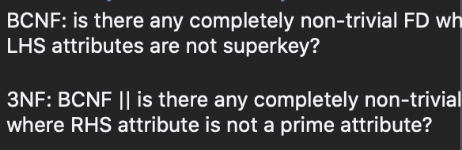
\includegraphics{images/b1}
\\\subsection*{Is \_\_ in BCNF}
1. Check if LHS not superkey (Use armstrong axiom if necessary)\\
\\\subsection*{Is \_\_ in 3NF}
\\
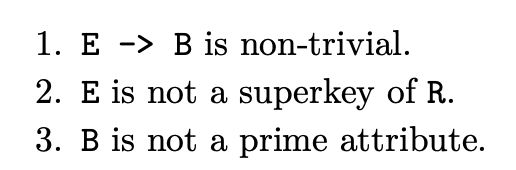
\includegraphics[height=1.5cm]{images/b5}\\
LHS not superkey and RHS not prime attribute
\\\\
\subsection*{Is all fragment in BCNF}\\
1. Calculate projection of decomposed fragments\\
2. Check if it belongs to any of the FD in the not decomposed schema\\\\
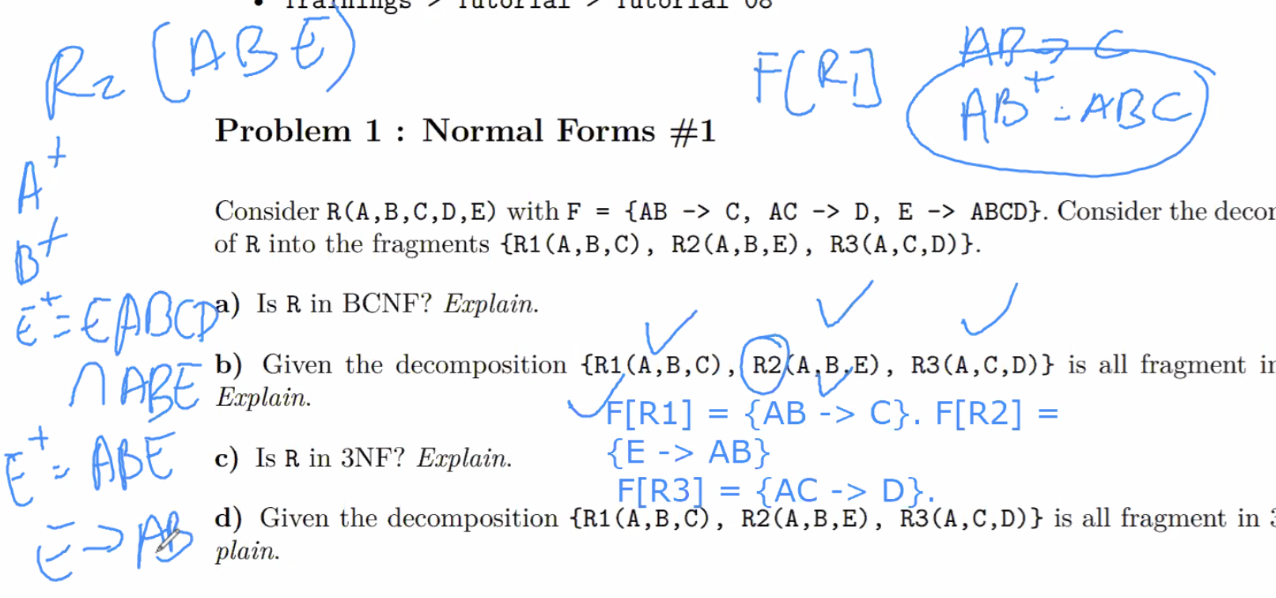
\includegraphics[height=5cm]{images/b2}
\subsection*{How to get prime attribute}\\
Compute the closure\\
Common mistake E $\rightarrow$ ABCD and E+ = ABCDE\\
\\
Prime attribute is the union of all possible keys
\\
\\
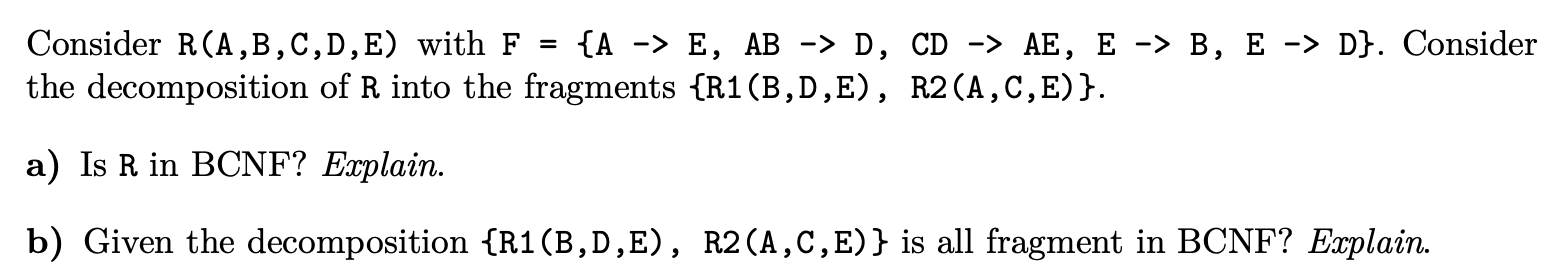
\includegraphics[height=2.5cm]{images/b3}\\
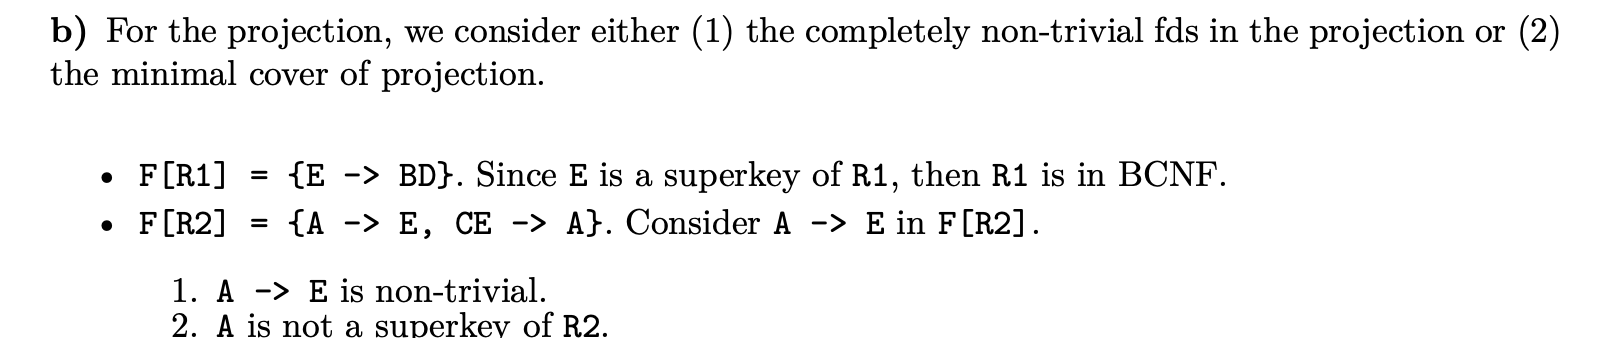
\includegraphics[height=3cm]{images/b4}
\vspace{0.5cm}
\\
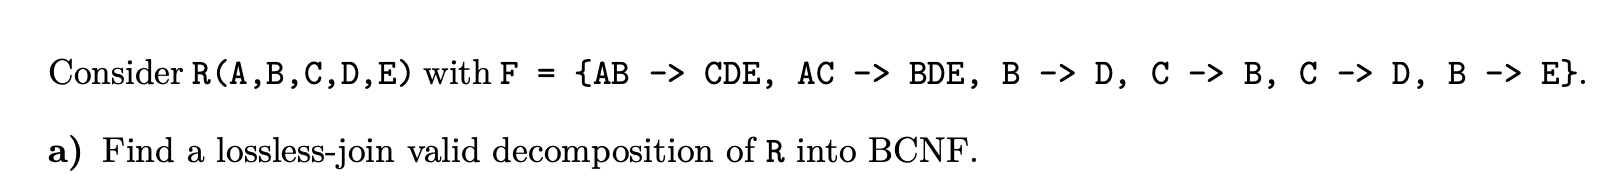
\includegraphics[height=1.5cm]{images/b7}\\
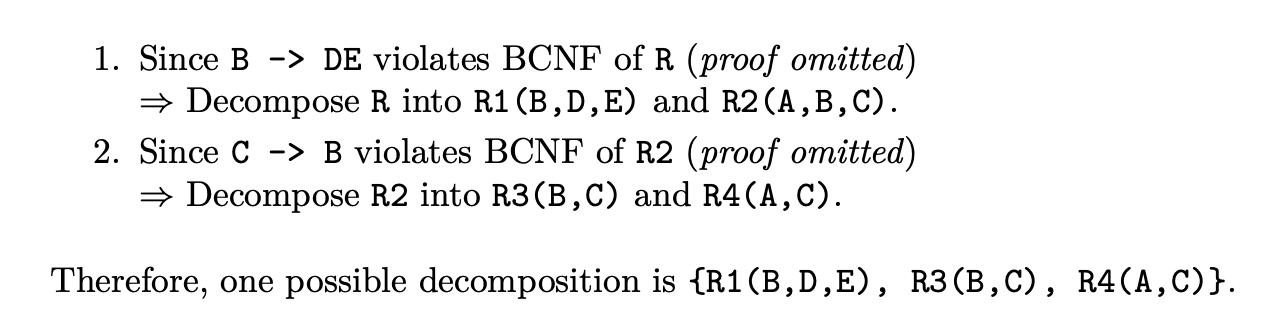
\includegraphics[height=3cm]{images/b6}
\\
\subsection*{Is lossless join}\\
1. Identify intersected attributes (can be a combination for eg. AB)\\
2. Get closure of intersected based on F\\
3. Check if any relation when intersected with the closure gives back the original relation
\\
\subsection*{Find BCNF decomposition}
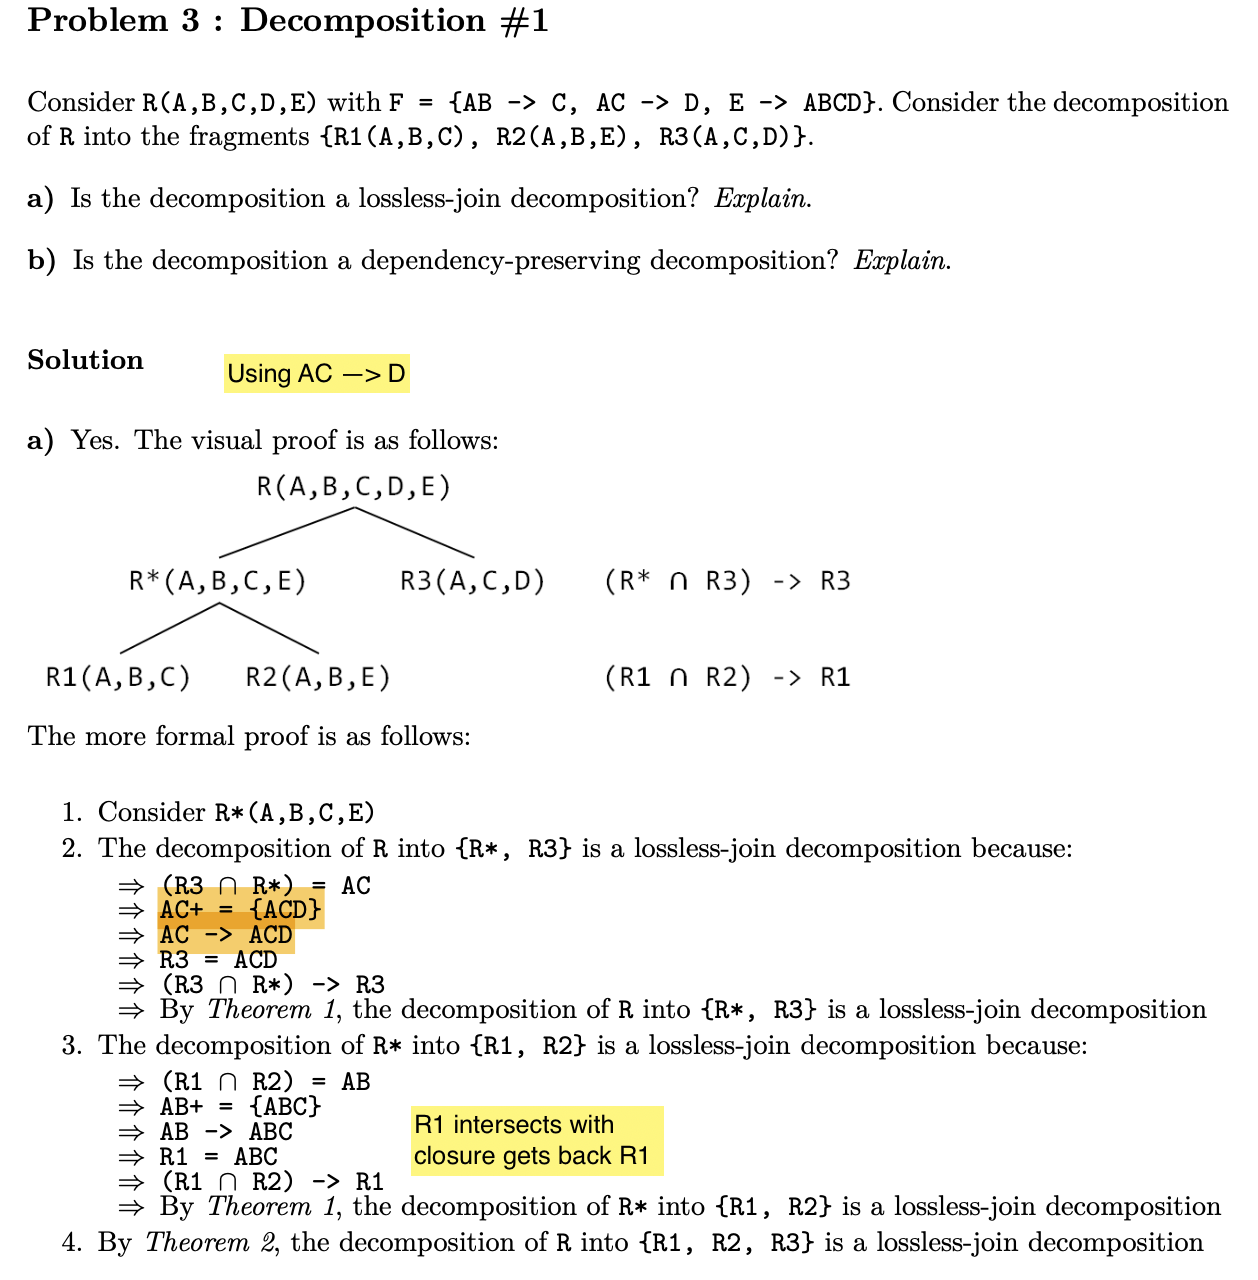
\includegraphics[height=10cm]{images/b8}
\subsection*{Is dp}\\
Only calculated the attribute closure of LHS attributes of F[R1]... F[Rn]\\
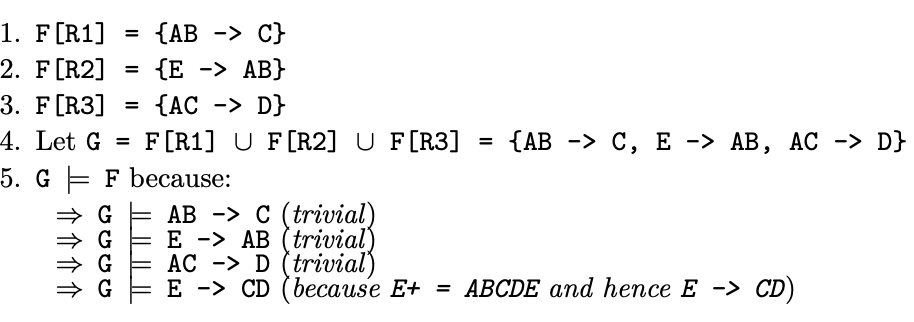
\includegraphics[height=3cm]{images/b9}
\subsection*{Minimum cover}\\
For each attribute on LHS, check if they are redundant and remove them\\
Consider R(A,B,C,D,E) with \\F = $\{AB \rightarrow CDE, AC  \rightarrow BDE, B  \rightarrow D, C  \rightarrow B, C  \rightarrow D, B  \rightarrow E\}$\\
Make sure all the Fds provided are logically implied
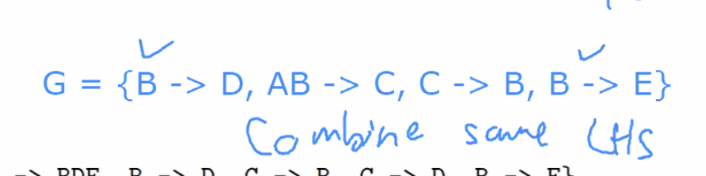
\includegraphics[height=1.5cm]{images/b11}
\subsection*{Find a lossless-join dependency-preserving valid decomposition of R into 3NF}\\
Use synthesis method\\
1. Find min cover\\
2. Combine same LHS\\
3. Combine into attributes of FD into schemas\\
4. Add key to schema\\
5. Remove redundant schemas (subset of other schemas)\\
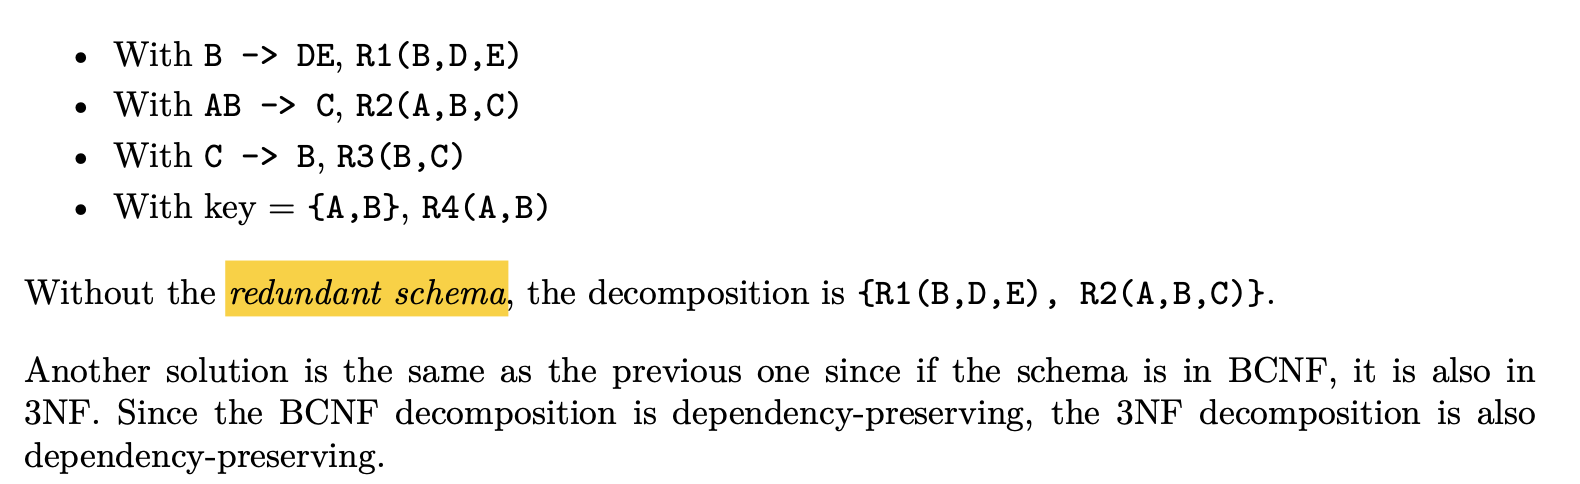
\includegraphics[height=3cm]{images/b12}
\subsection*{Armstrong axioms}
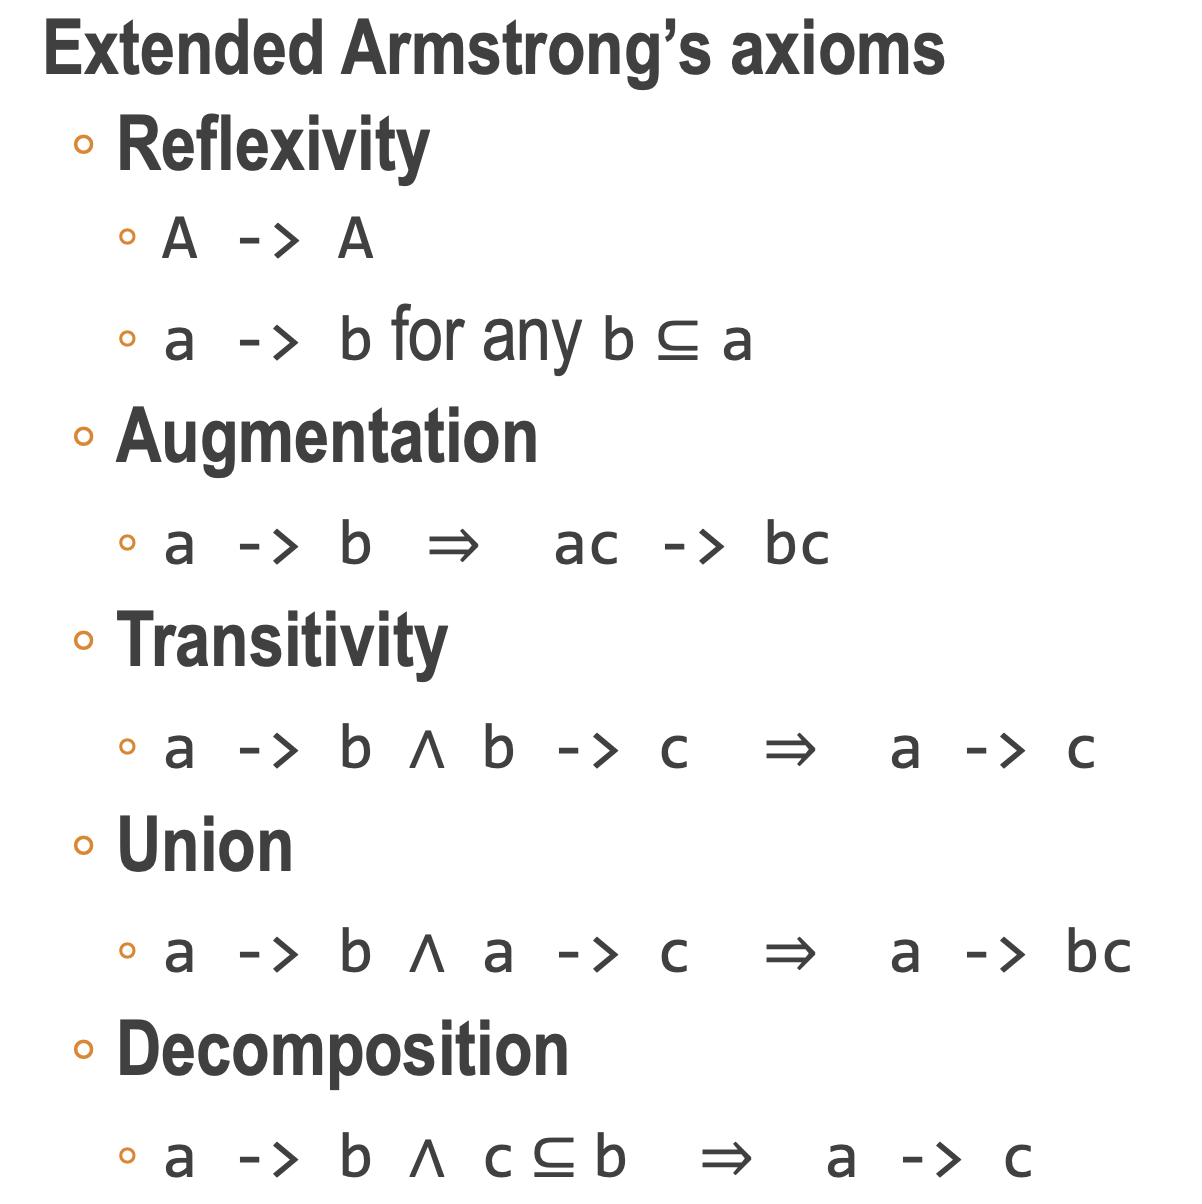
\includegraphics[height=3cm]{images/b13}
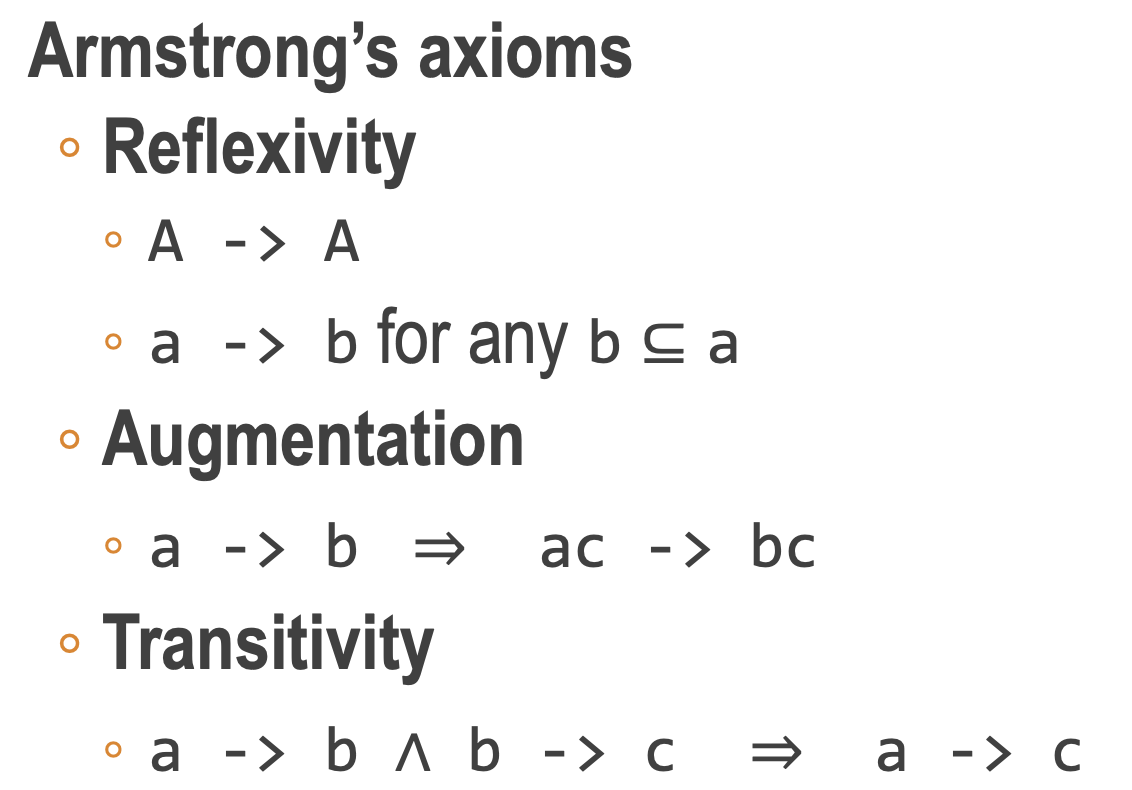
\includegraphics[height=3cm]{images/b14}\\
 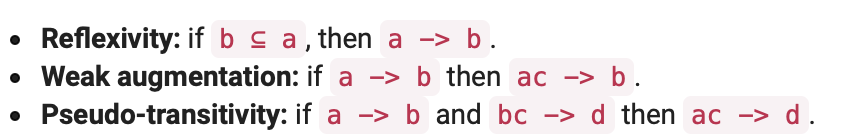
\includegraphics[height=1cm]{images/b16}
\subsection*{ISA}
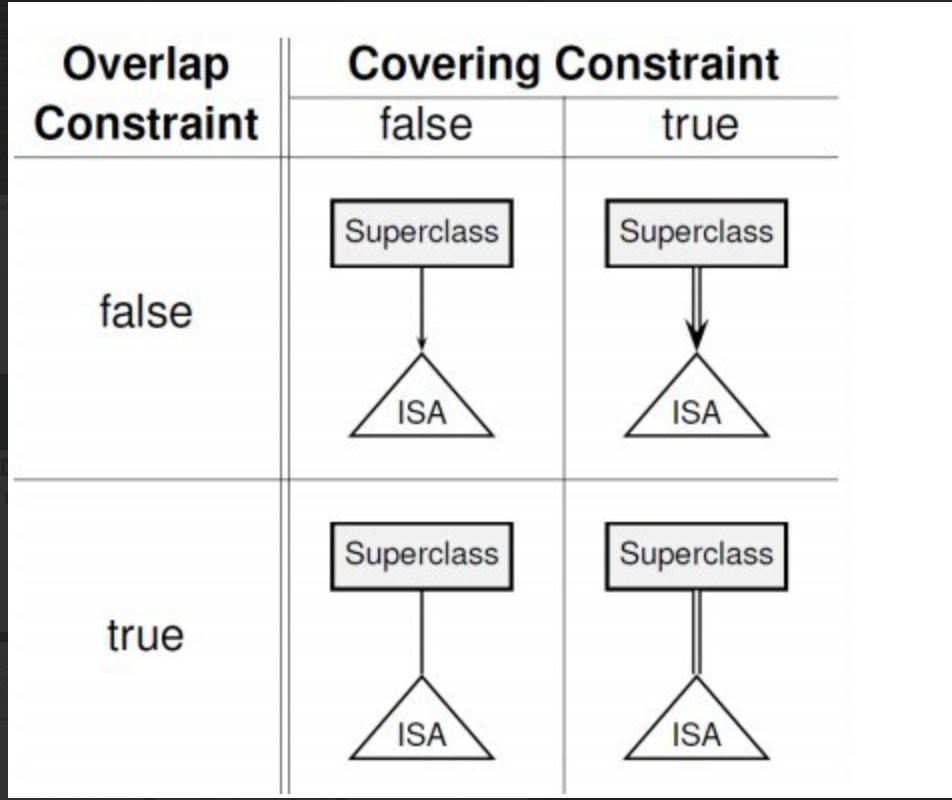
\includegraphics[height=3cm]{images/b15}
\subsection*{ER}
entA $\rightarrow$ ent\\
entA can uniquely identify all other entities\\
\\
\subsection*{Relational schema}\\
If the primary key of R consist of the primary of another entity, then there is total participation in both entities\\
Otherwise it is unconstrained
\end{multicols*}

\end{document}
